% Synthetic acceptance fixture (MIT, part of rstex2word). It mirrors the
% constructs of an amsart economics manuscript that tex2word 2.2.0 mangled:
% a \paragraph redefined through \@startsection, \subjclass[JEL], citations
% and \ref inside table cells, figure captions and theorem-like blocks, a
% landscape table built as \rotatebox{90}{minipage + \captionof{table}} with
% \makecell headers, and display math with sums, cases/align row spacing,
% \DeclareMathOperator and \mathrm words.
\documentclass[11pt,reqno]{amsart}
\usepackage{amsmath,amssymb,amsthm,mathtools}
\usepackage{booktabs,array,tabularx,longtable,makecell}
\usepackage{graphicx,xcolor,listings,caption}
\usepackage[authoryear,round]{natbib}
\usepackage{hyperref}
\newcolumntype{L}[1]{>{\raggedright\arraybackslash}p{#1}}
\newcolumntype{Y}{>{\raggedright\arraybackslash}X}

% amsart repurposed: JEL codes in \subjclass, bold run-in \paragraph heads
\makeatletter
\@namedef{subjclassname@JEL}{JEL classification}
\def\paragraph{\@startsection{paragraph}{4}\z@{0.6\baselineskip}{-\fontdimen2\font}{\normalfont\bfseries}}
\makeatother

\newcommand{\Gmin}{G^{\min}}
\DeclareMathOperator{\rel}{rel}
\theoremstyle{definition}
\newtheorem{designrule}{Design rule}

\begin{document}

\title[Fixture]{An amsart acceptance fixture: tables, captions and sums}
\author{A. Author}
\email{author@example.org}
\thanks{The code is listed in Appendix~\ref{app:code}.}
\keywords{acceptance test; amsart; behavioural model}
\subjclass[JEL]{D91, E21, J63}

\begin{abstract}
A small paper whose references live in table cells and captions.
\end{abstract}

\maketitle

\section{Model}\label{sec:model}

\paragraph{Reference-dependent adoption \citep{tk1991}.}
Adoption follows the share of exposed tasks, drawn from a
$\mathrm{Beta}(2,3)$ distribution; Table~\ref{tab:priors} lists the priors
and Section~\ref{sec:calib} their basis. The displaced share is
\begin{equation}\label{eq:share}
D_t = \frac{\sum_{i \in A_t} e_i\, \sigma}{\sum_i e_i},
\qquad
\Delta C = \bar m\,\Delta Y + \sum_k (m_k - \bar m)\,\Delta Y_k ,
\end{equation}
and the buffer inflow is
\begin{equation}\label{eq:inflow}
\alpha_t = \begin{cases} \min\!\left(\tfrac{1}{2}\Delta D_t,\; (B_{t-1} - 4 b_{t-1})^{+}\right) & B_{t-1} > 0, \\[2pt] 0 & B_{t-1} \le 0, \end{cases}
\end{equation}
with the stocks updated as
\begin{align}
b_t &= b_{t-1} + \alpha_t - \rel_t, \\[4pt]
G_t &= \frac{C_t}{C_0} - \frac{Y_t}{Y_0}, \qquad \Gmin = \min_t G_t. \label{eq:gap}
\end{align}

\begin{designrule}\label{rule:levy}
Finance the buffer from the margin, as present-biased households
\citep{laibson1997} consume transfers at once.
\end{designrule}

\begin{table}[tb]
\centering
\caption{Behavioural parameters and priors.}\label{tab:priors}
\begin{tabularx}{\textwidth}{@{}L{3.2cm}L{2.0cm}Y@{}}
\toprule
Parameter & Prior & Basis \\
\midrule
Loss aversion $\lambda$ & $U(1.5,\,3.0)$ & Around the \citet{tk1991} estimate \\
Present bias $\beta$ & $U(0.6,\,0.9)$ & \citet{laibson1997}; see Section~\ref{sec:calib} \\
\bottomrule
\end{tabularx}
\end{table}

\begin{longtable}{@{}L{3cm}L{6cm}@{}}
\caption{Sources.}\label{tab:sources}\\
\toprule
Source & Reference \\
\midrule
\endhead
Survey & \citet{laibson1997} \\
Model & Design rule~\ref{rule:levy} and \citep{tk1991} \\
\bottomrule
\end{longtable}

\begin{figure}[tb]
\centering
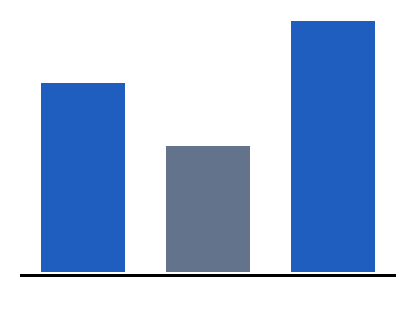
\includegraphics[width=0.6\textwidth]{figures/bars.pdf}
\caption{Adoption paths (source: \citealp{tk1991}).}\label{fig:bars}
\end{figure}

Figure~\ref{fig:bars} and Table~\ref{tab:results} report the scenarios.

\begin{table}[p]
\centering
\rotatebox{90}{\begin{minipage}{0.9\textheight}
\captionof{table}{Stress-test results; $\Gmin$ is defined in equation~\eqref{eq:gap}.}\label{tab:results}
\centering\scriptsize
\begin{tabular}{@{}lcr@{}}
\toprule
Scenario & \makecell[c]{Peak junior\\unemployment} & \makecell[r]{Consumption\\trough} \\
\midrule
S0 Baseline & 9.2 [6.7, 13.6] & $-1.82$\% \\
S1 Acceleration & 10.4 [7.1, 14.8] & $-1.91$\% \\
\bottomrule
\end{tabular}
\end{minipage}}
\end{table}

\section{Calibration}\label{sec:calib}
Calibrations follow \citet{laibson1997} and Design rule~\ref{rule:levy}.

\bibliographystyle{plainnat}
\bibliography{refs}

\appendix
\section{Model code}\label{app:code}
\lstinputlisting[language=Python]{model.py}

\end{document}
